\documentclass[DaoFP]{subfiles}
\begin{document}
\setcounter{chapter}{21}

\chapter{Dependent Types}

We've seen types that depend on other types. They are defined using type constructors with type parameters, like \hask{Maybe} or \hask{[]}. Most programming languages have some support for generic data types---data types parameterized by other data types.

Categorically, such types are modeled as functors \footnote{A type constructor that has no \hask{Functor} instance can be thought of as a functor from a discrete category---a category with no arrows other than identities}.

A natural generalization of this idea is to have types that are parameterized by values. For instance, it's often advantageous to encode the length of a list in its type. A list of length zero would have a different type than a list of length one, and so on. 

Obviously, you cannot change the length of such a list, since it would change its type. This is not a problem in functional programming, where all data types are immutable anyway. When you prepend an element to a list, you create a new list, at least conceptually. With a length-encoded list, this new list is of a different type, that's all!

Types parameterized by values are called \emph{dependent types}. There are languages like Idris or Agda that have full support for dependent types. It's also possible to implement dependent types in Haskell, but support for them is still rather patchy. 

The reason for using dependent types in programming is to make programs provably correct. In order to do that, the compiler must be able to check the assumptions made by the programmer. 

Haskell, with its strong type system, is able to uncover a lot of bugs at compile time. For instance, it won't let you write \hask{a <> b} (infix notation for \hask{mappend}), unless you provide the \hask{Monoid} instance for the type of your variables. 

However, within Haskell's type system, there is no way to express or, much less enforce, the unit and associativity laws for the monoid. For that, the instance of the \hask{Monoid} type class would have to carry with itself proofs of equality (not actual code):
\begin{haskell}
assoc :: m <> (n <> p) = (m <> n) <> p
lunit :: mempty <> m = m
runit :: m <> mempty = m
\end{haskell}
Dependent types, and equality types in particular, pave the way towards this goal.

The material in this chapter is more advanced, and not used in the rest of the book, so you may safely skip it on first reading. Also, to avoid confusion between fibers and functions, I decided to use capital letters for objects in parts of this chapter.

\section{Dependent Vectors}

We'll start with the standard example of a counted list, or a vector:
\begin{haskell}
data Vec n a where
    VNil  :: Vec Z a
    VCons :: a -> Vec n a -> Vec (S n) a
\end{haskell}
The compiler will recognize this definition as dependently typed if you include the following language pragmas:
\begin{haskell}
{-# LANGUAGE DataKinds #-}
{-# LANGUAGE GADTs #-}
\end{haskell}
The first argument to the type constructor is a natural number \hask{n}. Notice: this is a value, not a type. The type checker is able to figure this out from the usage of \hask{n} in the two data constructors. The first one creates a vector of the type \hask{Vec Z a}, and the second creates a vector of the type \hask{Vect (S n) a}, where \hask{Z} and \hask{S} are defined as the constructors of natural numbers:
\begin{haskell}
data Nat = Z | S Nat
\end{haskell}

We can be more explicit about the parameters if we use the pragma:
\begin{haskell}
{-# LANGUAGE KindSignatures #-}
\end{haskell}
and import the library:
\begin{haskell}
import Data.Kind
\end{haskell}
We can then specify that \hask{n} is a \hask{Nat}, whereas \hask{a} is a \hask{Type}:
\begin{haskell}
data Vec (n :: Nat) (a :: Type) where
    VNil  :: Vec Z a
    VCons :: a -> Vec n a -> Vec (S n) a
\end{haskell}

Using one of these definitions we can, for instance, construct a vector (of integers) of length zero:
\begin{haskell}
emptyV :: Vec Z Int
emptyV = VNil
\end{haskell}
It has a different type than a vector of length one:
\begin{haskell}
singleV :: Vec (S Z) Int
singleV = VCons 42 VNil
\end{haskell}
and so on.

We can now define a dependently typed function that returns the first element of a vector:
\begin{haskell}
headV :: Vec (S n) a -> a
headV (VCons a _) = a
\end{haskell}
This function is guaranteed to work exclusively with non-zero-length vectors. These are the vectors whose size matches \hask{(S n)}, which cannot be \hask{Z}. If you try to call this function with \hask{emptyV}, the compiler will flag the error.

Another example is a function that zips two vectors together. Encoded in its type signature is the requirement that the two vectors be of the same size \hask{n} (the result is also of the size \hask{n}):
\begin{haskell}
zipV :: Vec n a -> Vec n b -> Vec n (a, b)
zipV (VCons a as) (VCons b bs) = VCons (a, b) (zipV as bs)
zipV VNil VNil = VNil
\end{haskell}

Dependent types are especially useful when encoding the shapes of containers. For instance, the shape of a list is encoded in its length. A more advanced example would encode the shape of a tree as a runtime value.  

\begin{exercise}
Implement the function \hask{tailV} that returns the tail of the non-zero-length vector. Try calling it with \hask{emptyV}.
\end{exercise}

\section{Dependent Types Categorically}

The easiest way to visualize dependent types is to think of them as families of types indexed by elements of a set. In the case of counted vectors, the indexing set would be the set of natural numbers $\mathbb{N}$.

The zeroth type would be the unit type \hask{()} representing an empty vector. The type corresponding to \hask{(S Z)} would be \hask{a}; then we'd have a pair \hask{(a, a)}, a triple \hask{(a, a, a)} and so on, with higher and higher powers of \hask{a}.

If we want to talk about the whole family as one big set, we can take the sum of all these types. For instance, the sum of all powers of $a$ is the familiar list type, a.k.a., a free monoid:
\[ \mathit{List} (a) = 1 + a + a \times a + a \times a \times a + ... =  \sum_{n:\mathbb{N}} a^n \]

\subsection{Fibrations}

Although intuitively easy to visualize, this point of view doesn't generalize nicely to category theory, where we don't like mixing sets with objects. So we turn this picture on its head and instead of talking about injecting family members into the sum, we consider a mapping that goes in the opposite direction. 

This, again, we can first visualize using sets. We have one big set $E$ describing the \emph{entire} family, and a function $p$ called the projection, or a \index{display map}\emph{display map}, that goes from $E$ down to the indexing set $B$ (also called the \emph{base}). 

This function will, in general, map multiple elements to one. We can then talk about the inverse image of a particular element $x \in B$ as the set of elements that get mapped down to it by $p$. This set is called the \index{fiber}\emph{fiber} and is written $p^{-1} x$ (even though, in general, $p$ is not invertible in the usual sense). Seen as a collection of fibers, $E$ is often called a \emph{fiber bundle} or just a bundle.

\[
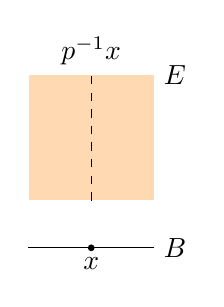
\begin{tikzpicture}

\def\yb{0}; % base
\def\yfb{0.6}; % fiber bottom
\def\yft{2.2}; % fiber top

\def\dx{0.8};

\def\xbl{0};
\def\xbm{\xbl + \dx};
\def\xbr{\xbl + 2*\dx};

\filldraw[fill=orange!30, draw=white] (\xbl, \yfb) rectangle (\xbr, \yft);

\draw (\xbl, \yb) -- (\xbr, \yb);

\draw[dashed] (\xbm, \yfb) -- (\xbm, \yft);

\filldraw[black] (\xbm, \yb) circle (1 pt);
\node[below] at (\xbm, \yb) {$x$};
\node[above] at (\xbm, \yft) {$p^{-1} x$};
\node[right] at (\xbr, \yb) {$B$};
\node[right] at (\xbr, \yft) {$E$};

\end{tikzpicture}
\]


Now forget about sets. A \emph{fibration} in an arbitrary category is a pair of objects $e$ and $b$ and an arrow $p \colon e \to b$. 

So this is really just an arrow, but the context is everything. When an arrow is called a fibration, we use the intuition from sets, and imagine its source $e$ as a collection of fibers, with $p$ projecting each fiber down to a single point in the base $b$. 

We can go even further: since (small) categories form a category $\mathbf{Cat}$ with functors as arrows, we can define a fibration of a category, taking another category as its base. 

\subsection{Type families as fibrations}

We will therefore model type families as fibrations. For instance, our counted-vector family can be represented as a fibration whose base is the type of natural numbers. The whole family is a sum (coproduct) of consecutive powers (products) of $a$:
\[ \mathit{List}(a) = a^0 + a^1 + a^2 + ... = \sum_{n\colon \mathbb{N}} a^n \]
with the zeroth power---the initial object---representing the vector of size zero.
\[
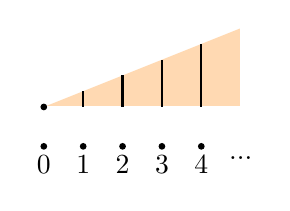
\begin{tikzpicture}
\def\dx{0.5};
\def\yb{0};
\def\dy{0.2};
\def\y{0.5};

\filldraw[fill=orange!30, draw=white] (0, \y) to (5* \dx, \y) to (5*\dx, \y + 5*\dy);

\filldraw[black] (0, 0) circle (1 pt);
\node[below] at (0, 0) {$0$};
\filldraw[black] (0, \y) circle (1 pt);

\filldraw[black] (\dx, 0) circle (1 pt);
\node[below] at (\dx, 0) {$1$};
\draw[thick] (\dx, \y) -- (\dx, \y + \dy);

\filldraw[black] (2*\dx, 0) circle (1 pt);
\node[below] at (2*\dx, 0) {$2$};
\draw[thick] (2*\dx, \y) -- (2*\dx, \y + 2* \dy);

\filldraw[black] (3*\dx, 0) circle (1 pt);
\node[below] at (3*\dx, 0) {$3$};
\draw[thick] (3*\dx, \y) -- (3*\dx, \y + 3* \dy);

\filldraw[black] (4*\dx, 0) circle (1 pt);
\node[below] at (4*\dx, 0) {$4$};
\draw[thick] (4*\dx, \y) -- (4*\dx, \y + 4* \dy);
\node[below] at (5*\dx, 0) {$...$};

\end{tikzpicture}
\]

The projection $p \colon \mathit{List}(a) \to \mathbb{N}$ is the familiar $\mathit{length}$ function. 

In category theory we like to describe things in bulk---defining internal structure of things by structure-preserving maps between them. Such is the case with fibrations. If we fix the base object $b$ and consider all possible source objects in the category $\mathcal{C}$, and all possible projections down to $b$, we get a \emph{slice category} $\mathcal{C}/b$. This category represents all the ways we can slice the objects of $\cat C$ over the base $b$.

Recall that the objects in the slice category are pairs $\langle e, p \colon e \to b \rangle$, and a morphism between two objects $\langle e, p \rangle$ and $\langle e', p' \rangle$ is an arrow $f \colon e \to e'$ that commutes with the projections, that is:
\[p' \circ f = p \]
The best way to visualize this is to notice that such a morphism maps fibers of $p$ to fibers of $p'$. It's a ``fiber-preserving'' mapping between bundles.

\[
 \begin{tikzcd}
 e
 \arrow[rd, "p"']
 \arrow[rr, "f"]
 && e'
 \arrow[ld, "p'"]
 \\
 &b
  \end{tikzcd}
\]

Our counted vectors can be seen as objects in the slice category $\mathcal{C}/\mathbb{N}$ given by pairs $\langle \mathit{List}(a), \mathit{length} \rangle$. A morphism in this category maps vectors of length $n$ to vectors of the same length $n$.

\subsection{Pullbacks}

We've seen a lot of examples of commuting squares. Such a square is a graphical representation of an equation: two path between opposite corners of a square, each a result of a composition of two morphisms, are equal. 

Like with every equality we may want to replace one or more of its components with an unknown, and try to solve the resulting equation. For instance, we may ask the question: Is there an object together with two arrows that would complete a commuting square? If many such objects exist, is there a universal one? If the missing piece of the puzzle is the upper left corner of a square (the source), we call it a pullback. If it's the lower right corner (the target), we call it a \index{pushout}pushout.

\[
 \begin{tikzcd}
 \color{red}?
 \arrow[d, red, dashed, "?"']
 \arrow[r, red, dashed, "?"]
 & E
 \arrow[d, "p"]
 \\
 A
 \arrow[r, "f"]
 &B
\end{tikzcd}
\hspace{40pt}
\begin{tikzcd}
 E
 \arrow[d, "p"']
 \arrow[r, "f"]
 & E'
 \arrow[d, red, dashed, "?"]
 \\
 B
 \arrow[r, red, dashed, "?"]
 &\color{red}?
 \end{tikzcd}
\]


 Let's start with a particular fibration $p \colon E \to B$ and ask ourselves the question: what happens when we change the base from $B$ to some $A$ that is related to it through a mapping $f \colon A \to B$. Can we ``pull the fibers back'' along $f$? 
 
 Again, let's think about sets first. Imagine picking a fiber in $E$ over some point $y \in B$ that is in the image of $f$. If $f$ were invertible, there would be an element $x = f^{-1} y$. We'd plant our fiber over it. In general, though, $f$ is not invertible. It means that there could be more elements of $A$ that are mapped to our $y$. In the picture below you see two such elements, $x_1$ and $x_2$. We'll just duplicate the fiber above $y$ and plant it over all elements that map to $y$. This way, every point in $A$ will have a fiber sticking out of it. The sum of all these fibers will form a new bundle $E'$.
 

\[
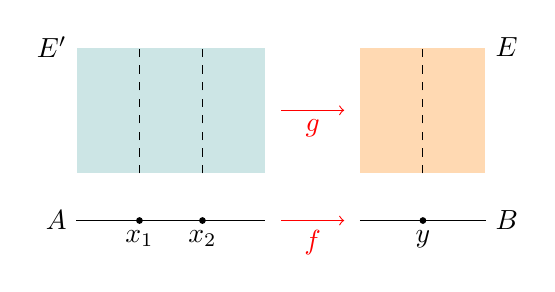
\begin{tikzpicture}

\def\yb{0}; % base
\def\yfb{0.6}; % fiber bottom
\def\yft{2.2}; % fiber top
\def\yfm{1.4} % fiber middle

\def\dx{0.8};

\def\xal{-1.8};
\def\xam{\xal + \dx};
\def\xamm{\xal + 2 * \dx};
\def\xar{\xal + 3*\dx};

\def\xbl{1.8};
\def\xbm{\xbl + \dx};
\def\xbr{\xbl + 2*\dx};

\filldraw[fill=blue!50!green!20, draw=white] (\xal, \yfb) rectangle (\xar, \yft);
\filldraw[fill=orange!30, draw=white] (\xbl, \yfb) rectangle (\xbr, \yft);

\draw (\xal, \yb) -- (\xar, \yb);
\draw (\xbl, \yb) -- (\xbr, \yb);

\draw[dashed] (\xam, \yfb) -- (\xam, \yft);
\draw[dashed] (\xamm, \yfb) -- (\xamm, \yft);
\draw[dashed] (\xbm, \yfb) -- (\xbm, \yft);

\filldraw[black] (\xam, \yb) circle (1 pt);
\filldraw[black] (\xamm, \yb) circle (1 pt);
\filldraw[black] (\xbm, \yb) circle (1 pt);
\node[below] at (\xbm, \yb) {$y$};
\node[right] at (\xbr, \yb) {$B$};
\node[left] at (\xal, \yb) {$A$};
\node[right] at (\xbr, \yft) {$E$};
\node[left] at (\xal, \yft) {$E'$};
\node[below] at (\xam, \yb) {$x_1$};
\node[below] at (\xamm, \yb) {$x_2$};

\draw[->, red] (\xar + 0.2, \yb) -- (\xbl - 0.2, \yb) node [midway, below] {$f$};
\draw[->, red] (\xar + 0.2, \yfm) -- (\xbl - 0.2, \yfm) node [midway, below] {$g$};

\end{tikzpicture}
\]

We have thus constructed a new fibration with the base $A$. Its projection $p' \colon E' \to A$ maps each point in a given fiber to the point over which this fiber was planted. There is also an obvious mapping $g \colon E' \to E$ that maps fibers to their corresponding fibers. 

By construction, this new fibration $\langle E', p'\rangle$ satisfies the condition:
\[ p \circ g = f \circ p' \]
which can be represented as a commuting square:
\[
 \begin{tikzcd}
 E'
 \arrow[d, "p'"']
 \arrow[r, "g"]
 & E
 \arrow[d, "p"]
 \\
 A
 \arrow[r, "f"]
 &B
  \end{tikzcd}
\]

In  $\mathbf{Set}$, we can explicitly construct $E'$ as a \emph{subset} of the cartesian product $A \times E$ with $p' = \pi_1$ and $g = \pi_2$ (the two cartesian projections). An element of $E'$ is a pair $\langle a, e \rangle$, such that:
\[ f (a) = p (e) \]

This commuting square is the starting point for the categorical generalization. However, even in $\mathbf{Set}$ there are many different fibrations over $A$ that make this diagram commute. We have to pick the universal one. Such a universal construction is called a \emph{pullback}, or a \emph{fibered product}.

In category theory, a \index{pullback}pullback of $p \colon e \to b$ along $f \colon a \to b$ is an object $e'$ together with two arrows $p' \colon e' \to a$ and $g \colon e' \to e$ that makes the following diagram commute\[
 \begin{tikzcd}
 &e'
 \arrow[r, "g"]
 \arrow[d, "p'"']
 &e
 \arrow[d, "p"]
 \\
 &a
 \arrow[r, "f"]
 &b
  \end{tikzcd}
\]
and that satisfies the universal condition. 


The universal condition says that, for any other candidate object $x$ with two arrows $q' \colon x \to e$ and $q \colon x \to a$ such that $p \circ q' = f \circ q$ (making the bigger ``square'' commute), there is a unique arrow $h \colon x \to e'$ that makes the two triangles commute, that is:
\begin{align*}
q &= p' \circ h \\
q' &= g \circ h
\end{align*}
Pictorially:
\[
 \begin{tikzcd}
 x
 \arrow[dr, dashed, "h"]
 \arrow[drr, bend left, "q'"]
 \arrow[ddr, bend right, "q"']
 \\
 &e'
 \arrow[r, "g"]
 \arrow[d, "p'"']
\arrow[dr, phantom,  , very near start, "\lrcorner"]
 &e
 \arrow[d, "p"]
 \\
 &a
 \arrow[r, "f"]
 &b
  \end{tikzcd}
\]
The angle symbol in the upper corner of the square is used to mark pullbacks.

If we look at the pullback through the prism of sets and fibrations, $e$ is a bundle over $b$, and we are constructing a new bundle $e'$ out of the fibers taken from $e$. Where we plant these fibers over $a$ is determined by (the inverse image of) $f$. This procedure makes $e'$ a bundle over both $a$ and $b$, the latter with the projection $p \circ g = f \circ p'$. 

The $x$ in this picture is some other bundle over $a$ with the projection $q$. It is simultaneously a bundle over $b$ with the projection $f \circ q = p \circ q'$. The unique mapping $h$ maps the fibers of $x$ given by $q^{-1}$ to fibers of $e'$ given by $p'^{-1}$. 

All mappings in this picture work on fibers. Some of them rearrange fibers over new bases---that's what a pullback does.  Other mappings modify individual fibers---the mapping $h \colon x \to e'$ works like this.

If you think of bundles as containers of fibers, the rearrangements of fibers corresponds to natural transformations, and the modifications of fibers correspond to the action of \hask{fmap}.
 
The universal condition then tells us that $q'$ can be factored into a modification of fibers $h$, followed by the rearrangement of fibers $g$.

It's worth noting that picking the terminal object or the singleton set as the pullback target gives us automatically the definition of the cartesian product:
\[
 \begin{tikzcd}
 b \times e
 \arrow[d, "\pi_1"']
 \arrow[r, "\pi_2"]
\arrow[dr, phantom,  , very near start, "\lrcorner"]
 & e
 \arrow[d, "!"]
 \\
 b
 \arrow[r, "!"]
 &
 1
  \end{tikzcd}
\]

Alternatively, we can think of this picture as planting as many copies of $e$ as there are elements in $b$. We'll use this analogy when we talk about the dependent sum and product.

Notice also that a single fiber can be extracted from a fibration by pulling it back to the terminal object. In this case the mapping $x \colon 1 \to b$ picks an element of the base, and the pullback along it extracts a single fiber $\varphi$:
\[
 \begin{tikzcd}
 \varphi
 \arrow[d, "!"']
 \arrow[r, "g"]
\arrow[dr, phantom,  , very near start, "\lrcorner"]
 & e
 \arrow[d, "p"]
 \\
 1
 \arrow[r, "x"]
 &
 b
  \end{tikzcd}
\]
The arrow $g$ injects this fiber back into $e$. By varying $x$ we can pick different fibers in $e$.

\begin{exercise}
Show that the pullback with the terminal object as the target is the product.
\end{exercise}
\begin{exercise}
Show that a pullback can be defined as a limit of the diagram from a stick-figure category with three objects:
\[ a \rightarrow b \leftarrow c \]
\end{exercise}

\begin{exercise}
Show that a pullback in $\mathcal{C}$ with the target $b$ is a product in the slice category $\mathcal{C}/b$. Hint: Define two projections  as morphisms in the slice category. Use universality of the pullback to show the universality of the product.
\end{exercise}

\subsection{Substitution}

We have two alternative descriptions of dependent types: one as fibrations and another as type families. It's in the latter framework that the pullback along a morphism $f$ can be interpreted as a substitution. When we have a type family $T y$ parameterized by elements $y \colon B$ and we always define a new type family by substituting $f x$ for $y$.

\[
 \begin{tikzcd}
 T (f x)
 & T y
 \\
 x
 \arrow[u, mapsto, ""]
 \arrow[r, mapsto, "f"]
 &y
 \arrow[u, mapsto, ""]
  \end{tikzcd}
\]
The new type family is thus parameterized by different shapes.

\subsection{Dependent environments}
When modeling lambda calculus, we used the objects of a cartesian closed category to serve both as types and environments. An empty environment was modeled as the terminal object (unit type), and we were building more complex environments using products. The order in which we multiply types doesn't matter since the product is symmetric (up to isomorphism).

When dealing with dependent types, we have to take into account that the type we are adding to the environment may depend on the values of the types already present in the environment. As before, we start with an empty environment modeled as the terminal object. 

\subsection{Weakening}

\subsection{Base-change functor}

We used a cartesian closed category as a model for programming. To model dependent types, we need to impose an additional condition: We require the category to be \index{locally cartesian closed category}\emph{locally cartesian closed}. This is a category in which all slice categories are cartesian closed. 

In particular, such categories have all pullbacks, so it's always possible to change the base of any fibration.  Base change induces a mapping between slice categories that is functorial. 

Given two slice categories $\mathcal{C}/b$ and $\mathcal{C}/a$ and an arrow between bases $f \colon b \to a$ the base-change functor $f^* \colon \mathcal{C}/a \to \mathcal{C}/b$ maps a fibration $\langle e, p \rangle$ to the fibration $ f^* \langle e, p \rangle= \langle f^* e, f^* p \rangle$, which is given by the pullback:
\[
 \begin{tikzcd}
f^* e
\arrow[dr, phantom,  , very near start, "\lrcorner"]
 \arrow[d, "f^*p"']
 \arrow[r, "g"]
 & e
 \arrow[d, "p"]
 \\
 b
 \arrow[r, "f"]
 &a
  \end{tikzcd}
\]
Notice that the functor $f^*$ goes in the opposite direction to the arrow $f$.

To visualize the base-change functor let's consider how it works on sets. 
\[
 \begin{tikzcd}
f^* E
\arrow[dr, phantom,  , very near start, "\lrcorner"]
 \arrow[d, "f^*p"']
 \arrow[r, "g"]
 & E
 \arrow[d, "p"]
 \\
 B
 \arrow[r, "f"]
 &A
  \end{tikzcd}
\]
We have the intuition that the fibration $p$ decomposes the set $E$ into fibers over each point of $A$. 

We can think of $f$ as another fibration that similarly decomposes $B$. Let's call these fibers in $B$ ``patches.'' For instance, if $A$ is just a two-element set, then the fibration given by $f$ splits $B$ into two patches. The pullback takes a fiber from $E$ and plants it over the whole patch in $B$. The resulting set $f^*E$ looks like a patchwork, where each patch is planted with clones of a single fiber from $E$.


\[
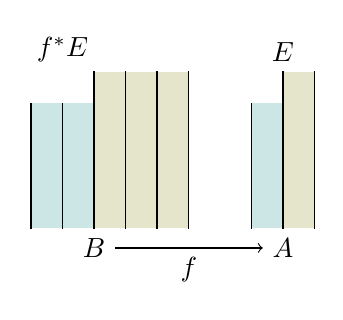
\begin{tikzpicture}
\def\xmin{1.4};
\def\dx{0.4};
\def\xl{-1.4};

\def\dy{0.2};
\def\yb{0};
\def\yt{10 * \dy}; 

% bars over A
\filldraw[fill=blue!50!green!20, draw=white] (\xmin, \yb) rectangle (\xmin + \dx, \yt - 2*\dy);
\filldraw[fill=red!50!green!20, draw=white] (\xmin + \dx, \yb) rectangle (\xmin + 2 * \dx, \yt);

\draw (\xmin, \yb) -- (\xmin, \yt - 2*\dy);
\draw (\xmin + \dx, \yb) -- (\xmin+ \dx, \yt);
\draw (\xmin + 2 * \dx, \yb) -- (\xmin + 2 * \dx, \yt);

\node[below] (BB) at (\xmin + \dx, \yb) {$A$};
\node[above] at (\xmin + \dx, 10 * \dy) {$E$};

% bars over B

\filldraw[fill=blue!50!green!20, draw=white] (\xl, \yb) rectangle (\xl + 5 * \dx, \yt - 2*\dy);
\filldraw[fill=red!50!green!20, draw=white] (\xl + 2*\dx, \yb) rectangle (\xl + 5 * \dx, \yt);
\draw (\xl, \yb) -- (\xl, \yt - 2*\dy);
\draw (\xl + \dx, \yb) -- (\xl + \dx, \yt - 2 * \dy);
\draw (\xl + 2 * \dx, \yb) -- (\xl + 2 * \dx, \yt);
\draw (\xl + 3 * \dx, \yb) -- (\xl + 3 * \dx, \yt);
\draw (\xl + 4 * \dx, \yb) -- (\xl + 4 * \dx, \yt);
\draw (\xl + 5 * \dx, \yb) -- (\xl + 5 * \dx, \yt);

\node[below] (B) at (\xl + 2 * \dx, \yb) {$B$};
\node[above] at (\xl + \dx, 10 * \dy) {$f^* E$};

\draw[->]  (B) -- (BB) node [midway, below] {$f$};


\end{tikzpicture}
\]

Since we have a function from $B$ to $A$ that may map many elements to one, the fibration over $B$ has finer grain than the coarser fibration over $A$. The simplest, least-effort way to turn the fibration of $E$ over $A$ to a fibration over $B$, is to spread the existing fibers over the patches defined by (the inverse of) $f$. This is the essence of the universal construction of the pullback.

In particular, if $A$ is a singleton set (the terminal object), then we have only one fiber (the whole of $E$) and the bundle $f^*E$ is a cartesian product $B \times E$. Such bundle is called a \index{trivial bundle}\emph{trivial bundle}.

A non-trivial bundle is not a product, but it can be \emph{locally} decomposed into products. Just as $B$ is a sum of patches, so $f^*E$ is a sum of products of these patches and the corresponding fibers of $E$.



You may also think of $A$ as providing an \emph{atlas} that enumerates all the patches in the \emph{base} $B$. Imagine that $A$ is a set of countries and $B$ is a set of cities. The mapping $f$ assigns a country to each city.

Continuing with this example, let $E$ be the set of languages fibrated by the country. If we assume that in each city the language of the given country is spoken, the base-change functor replants the country's languages over each of its cities.

By the way, this idea of using local patches and an atlas goes back to differential geometry and general relativity, where we often glue together local coordinate systems to describe topologically nontrivial bundles, like M\"{o}bius strips or Klein bottles.

As we'll see soon, in a locally cartesian closed category, the base change functor has both the left and the right adjoints. The left adjoint to $f^*$ is called $f_!$ (sometimes pronounced ``f down-shriek'') and the right adjoint is called $f_*$ (``f down-star''):
\[ f_! \dashv f^* \dashv f_* \]
In programming, the left adjoint is called the dependent sum, and the right adjoint is called the dependent product or dependent function:
\[ \Sigma_f \dashv f^* \dashv \Pi_f \]

\begin{exercise}
Define the action of the base-change functor on morphisms in $\cat C/a$, that is, given a morphism $h$ construct its counterpart $f^* h$
\[
 \begin{tikzcd}
f^* e'
 \arrow[dr, "f^*p'"']
 \arrow[r, red, "f^* h"]
 & f^* e
\arrow[d, "f^*p"]
&& e'
\arrow[d, "p'"]
\arrow[r, red, "h"]
& e
\arrow[dl, "p"]
 \\
& b
\arrow[rr, "f"']
 &&a
\end{tikzcd}
\hspace{40pt}
\begin{tikzcd}
\end{tikzcd}
\]
Hint: Use the universality of the pullback and the commuting condition: $g' \circ h \circ p = f^* p' \circ f$.

\[
\begin{tikzcd}
 f^* e'
 \arrow[dr, dashed, red, "f^* h"]
 \arrow[drr, bend left, "g' \circ h"]
 \arrow[ddr, bend right, "f^* p'"']
 \\
 &f^* e
 \arrow[r, "g"]
 \arrow[d, "f^* p"']
\arrow[dr, phantom,  , very near start, "\lrcorner"]
 &e
 \arrow[d, "p"]
 \\
 &b
 \arrow[r, "f"]
 &a
\end{tikzcd}
\hspace{40pt}
\begin{tikzcd}
f^* e'
\arrow[r, "g'"]
\arrow[d, "f^* p'"']
\arrow[dr, phantom,  , very near start, "\lrcorner"]
& e'
\arrow[d, "p'"']
\arrow[r, red, "h"]
& e
\arrow[dl, "p"]
\\
b
\arrow[r, "f"]
& a
\end{tikzcd}
\]


\end{exercise}

\section{Dependent Sum}

In type theory, the dependent sum, or the sigma type $\Sigma_{x : B} T(x)$, is defined as a type of pairs in which the \emph{type} of the second component depends on the \emph{value} of the first component. 

Conceptually, the sum type is defined using its mapping-out property. The mapping out of a sum is a pair of mappings, as illustrated in this adjunction:
\[ \mathcal{C}(F_1 + F_2, F) \cong (\mathcal{C} \times \mathcal{C}) (\langle F_1, F_2 \rangle, \Delta F) \]
Here, we have a pair of arrows $(F_1 \to F, F_2 \to F)$ that define the mapping out of the sum $S = F_1 + F_2$. In $\Set$, the sum is a tagged union. A dependent sum is a sum that is tagged by elements of another set.

Our counted vector type can be thought of as a dependent sum tagged by natural numbers. An element of this type is a natural number \hask{n}  (a value) paired with an element of the n-tuple type \hask{(a, a, ... a)}. Here are some counted vectors of integers written in this representation:
\begin{haskell}
(0, ())
(1, 42)
(2, (64, 7))
(5, (8, 21, 14, -1, 0))
\end{haskell}

More generally, the introduction rule for the dependent sum assumes that there is a family of types $T(x)$ indexed by elements of the base type $B$. Then an element of $\Sigma_{x : B} T(x)$ is constructed from a pair of elements $x \colon B$ and $y \colon T(x)$. 

Categorically, dependent sum is modeled as the left adjoint of the base-change functor. 

To see this, let's first revisit the definition of a pair, which is an element of a product. We've noticed before that a product can be written as a pullback from the singleton set---the terminal object. Here's the universal construction for the product/pullback (the notation anticipates the target of this construction):
\[
 \begin{tikzcd}
 S
 \arrow[dr, blue, dashed, "\phi^T"]
 \arrow[drr, blue, bend left, "\phi"]
 \arrow[ddr, bend right, "q"]
 \\
 &B \times F
\arrow[dr, phantom,  , very near start, "\lrcorner"]
 \arrow[r, "\pi_2"]
 \arrow[d, "\pi_1"']
 &F
 \arrow[d, "!"]
 \\
 &B
 \arrow[r, "!"]
 &1
  \end{tikzcd}
\]

We have also seen that the product can be defined using an adjunction. We can spot this adjunction in our diagram: for every pair of arrows $\langle \phi, q \rangle$ there is a unique arrow $\phi^T$ that makes the triangles commute. 

Notice that, if we keep $q$ fixed, we get a one-to-one correspondence between the arrows $\phi$ and $\phi^T$. This will be the adjunction we're interested in.

We can now put our fibrational glasses on and notice that $\langle S, q\rangle$ and $\langle B \times F, \pi_1 \rangle$ are two fibrations over the same base $B$. The commuting triangle makes $\phi^T$ a morphism in the slice category $\mathcal{C}/B$, or a fiber-wise mapping. In other words $\phi^T$ is a member of the hom-set:
 \[ (\mathcal{C}/B) \left(\left \langle {S \atop q} \right \rangle, \left \langle {B \times F \atop \pi_1} \right \rangle \right)  \]
 
 Since $\phi$ is a member of the hom-set $ \mathcal{C}(S, F)$, we can rewrite the one-to-one correspondence between $\phi^T$ and  $\phi$ as an isomorphism of hom-sets:
\[  (\mathcal{C}/B)\left(\left \langle {S \atop q} \right \rangle, \left \langle {B \times F \atop \pi_1} \right \rangle \right) \cong \mathcal{C}(S, F) \]
In fact, it's an adjunction in which we have the forgetful functor $U \colon \mathcal{C}/B \to \mathcal{C}$ mapping $\langle S, q \rangle$ to $S$, thus forgetting the fibration.

If you squint at this adjunction hard enough, you can see the outlines of the definition of $S$ as a categorical sum (coproduct). 

Firstly, on the right you have a mapping out of $S$. Think of $S$ as the sum of fibers that are defined by the fibration $\langle S, q \rangle$. 

Secondly, recall that the fibration $\langle B \times F, \pi_1 \rangle$ can be though of as producing many copies of $F$ planted over points in $B$. This is a generalization of the diagonal functor $\Delta$ that duplicates $F$---here, we make ``$B$ copies'' of $F$. The left hand side of the adjunction is just a bunch of arrows, each mapping a different fiber of $S$ to the target fiber $F$. 

\[
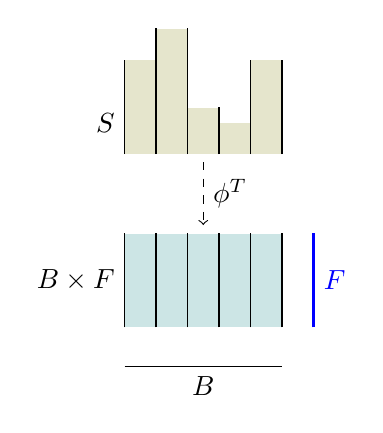
\begin{tikzpicture}
\def\xmin{1.4};
\def\dx{0.4};
\def\xl{-1.4};

\def\dy{0.2};
\def\yb{0.2};
\def\yt{10 * \dy}; 

\def\ybb{-2};
\def\ytt{\ybb + 6 * \dy};

\def\ybase{-2.5}

% bars above

\def\yya{\yt - 3 * \dy}
\def\yyb{\yt - 1 * \dy}
\def\yyc{\yt - 6 * \dy}
\def\yyd{\yt - 7 * \dy}

\filldraw[fill=red!50!green!20, draw=white] (\xl + 0*\dx, \yb) rectangle (\xl + 1 * \dx, \yya);
\filldraw[fill=red!50!green!20, draw=white] (\xl + 1*\dx, \yb) rectangle (\xl + 2 * \dx, \yyb);
\filldraw[fill=red!50!green!20, draw=white] (\xl + 2*\dx, \yb) rectangle (\xl + 3 * \dx, \yyc);
\filldraw[fill=red!50!green!20, draw=white] (\xl + 3*\dx, \yb) rectangle (\xl + 4 * \dx, \yyd);
\filldraw[fill=red!50!green!20, draw=white] (\xl + 4*\dx, \yb) rectangle (\xl + 5 * \dx, \yya);

\draw (\xl + 0 * \dx, \yb) -- (\xl + 0 * \dx, \yya);
\draw (\xl + 1 * \dx, \yb) -- (\xl + 1 * \dx, \yyb);
\draw (\xl + 2 * \dx, \yb) -- (\xl + 2 * \dx, \yyb);
\draw (\xl + 3 * \dx, \yb) -- (\xl + 3 * \dx, \yyc);
\draw (\xl + 4 * \dx, \yb) -- (\xl + 4 * \dx, \yya);
\draw (\xl + 5 * \dx, \yb) -- (\xl + 5 * \dx, \yya);


% bars below

\filldraw[fill=blue!50!green!20, draw=white] (\xl, \ybb) rectangle (\xl + 5 * \dx, \ytt);
\draw (\xl + 0 * \dx, \ybb) -- (\xl + 0 * \dx, \ytt);
\draw (\xl + 1 * \dx, \ybb) -- (\xl + 1 * \dx, \ytt);
\draw (\xl + 2 * \dx, \ybb) -- (\xl + 2 * \dx, \ytt);
\draw (\xl + 3 * \dx, \ybb) -- (\xl + 3 * \dx, \ytt);
\draw (\xl + 4 * \dx, \ybb) -- (\xl + 4 * \dx, \ytt);
\draw (\xl + 5 * \dx, \ybb) -- (\xl + 5 * \dx, \ytt);

\node[left] at (\xl, \ybb + 3 * \dy) {$B \times F$};
\node[left] at (\xl, 3 * \dy) {$S$};
\draw[thick, blue] (\xl + 6 * \dx, \ybb) -- (\xl + 6 * \dx, \ytt) node[midway, right] {$F$};
\draw[] (\xl, \ybase) -- (\xl + 5 * \dx, \ybase) node [midway, below] {$B$};

\draw[->, dashed] (\xl + 2.5 * \dx, \yb - 0.1) -- (\xl + 2.5 * \dx, \ytt + 0.1) node[midway, right] {$\phi^T$};

\end{tikzpicture}
\]

Applying this idea to our counted-vector example, $\phi^T$ stands for infinitely many functions, one per every natural number. In practice, we define these functions using recursion. For instance, here's a mapping out of a vector of integers:
\begin{haskell}
sumV :: Vec n Int -> Int
sumV VNil = 0
sumV (VCons n v) = n + sumV v
\end{haskell}

\subsection{Adding the atlas}

We can generalize our diagram by replacing the terminal object with an arbitrary base $A$ (an atlas). Instead of a single fiber, we now have a fibration $\langle F, p \rangle$, and we use the pullback square that defines the base-change functor $f^*$:
\[
 \begin{tikzcd}
 S
 \arrow[dr, blue, dashed, "\phi^T"]
 \arrow[drr, blue, bend left, "\phi"]
 \arrow[ddr, bend right, "q"]
 \\
 &f^* F
\arrow[dr, phantom,  , very near start, "\lrcorner"]
 \arrow[r, "g"]
 \arrow[d, "f^* p"']
 &F
 \arrow[d, "p"]
 \\
 &B
 \arrow[r, "f"]
 &A
  \end{tikzcd}
\]

We can imagine that the fibration over $B$ is finer grain, since $f$ may map multiple points to one. Think, for instance, of a function \hask{even :: Nat -> Bool} that creates two bunches of even and odd numbers. In this picture, $f$ defines a coarser ``resampling'' of the original $S$.

The universality of the pullback results in the following isomorphism of hom-sets:

\[  (\mathcal{C}/B) \left( \left \langle {S \atop q} \right \rangle , f^* \left \langle {F \atop p} \right \rangle \right) \cong (\mathcal{C}/A) \left( \left \langle {S \atop f \circ q } \right \rangle , \left \langle {F \atop p} \right \rangle \right)  \]
Here, $\phi^T$ is an element of the left-hand side, and $\phi$ is the corresponding element of the right-hand side. 

We interpret this isomorphism as the adjunction between the base change functor $f^*$ on the left and the dependent sum functor on the right. 
\[  (\mathcal{C}/B) \left( \left \langle {S \atop q} \right \rangle , f^* \left \langle {F \atop p} \right \rangle \right) \cong (\mathcal{C}/A) \left( \Sigma_f \left \langle {S \atop q} \right \rangle , \left \langle {F \atop p} \right \rangle \right)  \]
The dependent sum is thus given by this formula:
\[ \Sigma_f \left \langle {S \atop q} \right \rangle =  \left \langle {S \atop f \circ q} \right \rangle \]
This says that, if $S$ is fibered over $B$ using $q$, and there is a mapping $f$ from $B$ to $A$, then $S$ is automatically (more coarsely) fibered over $A$, the projection being the composition $f \circ q$. 

We've seen before that, in $\mathbf{Set}$, $f$ defines patches within $B$. Fibers of $F$ are replanted in these patches to form $f^*F$.  Locally---that is within each patch---$f^*F$ looks like a cartesian product. 

\[
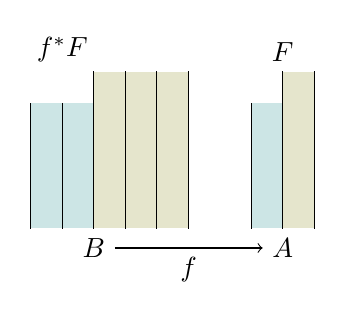
\begin{tikzpicture}
\def\xmin{1.4};
\def\dx{0.4};
\def\xl{-1.4};

\def\dy{0.2};
\def\yb{0};
\def\yt{10 * \dy}; 

% bars over A
\filldraw[fill=blue!50!green!20, draw=white] (\xmin, \yb) rectangle (\xmin + \dx, \yt - 2*\dy);
\filldraw[fill=red!50!green!20, draw=white] (\xmin + \dx, \yb) rectangle (\xmin + 2 * \dx, \yt);

\draw (\xmin, \yb) -- (\xmin, \yt - 2*\dy);
\draw (\xmin + \dx, \yb) -- (\xmin+ \dx, \yt);
\draw (\xmin + 2 * \dx, \yb) -- (\xmin + 2 * \dx, \yt);

\node[below] (BB) at (\xmin + \dx, \yb) {$A$};
\node[above] at (\xmin + \dx, 10 * \dy) {$F$};

% bars over B

\filldraw[fill=blue!50!green!20, draw=white] (\xl, \yb) rectangle (\xl + 5 * \dx, \yt - 2*\dy);
\filldraw[fill=red!50!green!20, draw=white] (\xl + 2*\dx, \yb) rectangle (\xl + 5 * \dx, \yt);
\draw (\xl, \yb) -- (\xl, \yt - 2*\dy);
\draw (\xl + \dx, \yb) -- (\xl + \dx, \yt - 2 * \dy);
\draw (\xl + 2 * \dx, \yb) -- (\xl + 2 * \dx, \yt);
\draw (\xl + 3 * \dx, \yb) -- (\xl + 3 * \dx, \yt);
\draw (\xl + 4 * \dx, \yb) -- (\xl + 4 * \dx, \yt);
\draw (\xl + 5 * \dx, \yb) -- (\xl + 5 * \dx, \yt);

\node[below] (B) at (\xl + 2 * \dx, \yb) {$B$};
\node[above] at (\xl + \dx, 10 * \dy) {$f^* F$};

\draw[->]  (B) -- (BB) node [midway, below] {$f$};


\end{tikzpicture}
\]
$S$ itself is fibered in two ways: coarsely chopped over $A$ using $f \circ q$ and finely julienned over $B$ using $q$. 

In category theory, the dependent sum, which is the left adjoint to the base change functor $f^*$, is denoted by $f_!$. For a given $f \colon b \to a$, it's a functor:
\[ f_! \colon \cat C/b \to \cat C/a \]
Its action on an object $(s, q \colon s \to b)$ is given by post-composition by $f$:
\[ f_! (s, q)= (s, f \circ q) \]

\subsection{Existential quantification}

In the \emph{propositions as types} interpretation, type families correspond to families of propositions. The dependent sum type $\Sigma_{x : B} \, T(x)$ corresponds to the proposition: There exists an $x$ for which $T(x)$ is true:
\[ \exists_{x : B} \, T (x)\]

Indeed, a term of the type $\Sigma_{x : B} \, T(x)$ is a pair of an element $x \colon B$ and an element $y \colon T(x)$---which shows that $T(x)$ is inhabited for some $x$.

\section{Dependent Product}

In type theory, the dependent product, or dependent function, or pi-type $\Pi_{x:B} T(x)$, is defined as a function whose return \emph{type} depends on the \emph{value} of its argument. 

It's called a function, because you can evaluate it. Given a dependent function  $f \colon \Pi_{x:B} T(x)$, you may apply it to an argument $x\colon B$ to get a value $f(x) \colon T(x)$.

\subsection{Dependent product in Haskell}
A simple example of a dependent product is a function that constructs a vector of a given size and fills it with copies of a given value:
\begin{haskell}
replicateV :: a -> SNat n -> Vec n a
replicateV _ SZ  = VNil
replicateV x (SS n) = VCons x (replicateV x n)
\end{haskell}

At the time of this writing, Haskell's support for dependent types is limited, so the implementation of dependent functions requires the use of singleton types. In this case, the number that is the argument to \hask{replicateV} is passed as a singleton natural:
\begin{haskell}
data SNat n where
  SZ :: SNat Z
  SS :: SNat n -> SNat (S n)
\end{haskell}
(Note that \hask{replicateV} is a function of two arguments, so it can be either considered a dependent function of a pair, or a regular function returning a dependent function.)
\subsection{Dependent product of sets}
Before we describe the categorical model of dependent functions, it's instructive to consider how they work on sets. A dependent function selects one element from each set $T(x)$. 

You may visualize the totality of this selection as a giant tuple---an element of a cartesian product. For instance, in the trivial case of $B$ a two-element set $\{1, 2\}$, a dependent function type is just a cartesian product $T(1) \times T(2)$. In general, you get one tuple component per every value of $x$. It's a giant tuple indexed by elements of $B$. This is the meaning of the product notation, $\Pi_{x:B} T(x)$. 

In our example, \hask{replicateV} picks a particular counted vector for each value of \hask{n}. Counted vectors are equivalent to tuples so, for \hask{n} equal zero, \hask{replicateV} returns an empty tuple \hask{()}; for \hask{n = 1} it returns a single value \hask{x}; for \hask{n} equal two, it duplicates \hask{x} returning \hask{(x, x)}; etc. 

The function \hask{replicateV}, evaluated at some \hask{x :: a},  is equivalent to an infinite tuple of tuples:
\[ ((), x, (x, x), (x, x, x), ...) \]
which is a specific element of the type:
\[ ((), a, (a, a), (a, a, a), ...) \]

\subsection{Dependent product categorically}
In order to build a categorical model of dependent functions, we need to change our perspective from a family of types to a fibration. We start with a bundle $E/B$ fibered by the projection $p\colon E \to B$. A dependent function is called a \emph{section} of this bundle. 

If you visualize the bundle as a bunch of fibers sticking out from the base $B$, a section is like a haircut: it cuts through each fiber to produce a corresponding value. In physics, such sections are called fields---with spacetime as the base. 

Just like we talked about a function object representing a set of functions, we can talk about an object $S(E)$ that represents a set of sections of a given bundle $E$. 

Just like we defined function application as a mapping out of the product:
\[\varepsilon_{B C} \colon C^B \times B \to C\]
we can define the dependent function application as a mapping:
\[\varepsilon \colon S(E) \times B \to E\]
We can visualize it as picking a section $s$ in $S(E)$ and an element $x$ of the base $B$ and producing a value in the bundle $E$. (In physics, this would correspond to measuring a field at a particular point in spacetime.)

But this time we have to insist that this value be in the correct fiber. If we project the result of applying $\varepsilon$ to $(s, x)$, it should fall back to the $x$. 

\[
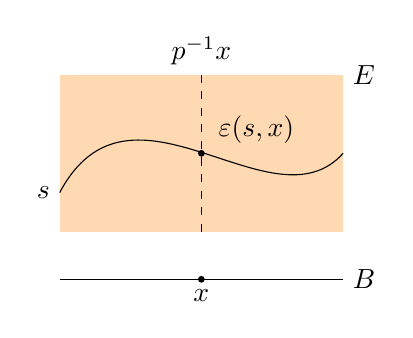
\begin{tikzpicture}

\def\dy{0.2};
\def\yb{-0.6}; % base
\def\yfb{0}; % fiber bottom
\def\yfs{0.5}; % s
\def\yfss{1.0}; % s'
\def\yft{2}; % fiber top

\def\dx{0.9};

\def\xbl{0};
\def\xbmr{\xbl + 2*\dx};
\def\xbr{\xbl + 4*\dx};

\filldraw[fill=orange!30, draw=white] (\xbl, \yfb) rectangle (\xbr, \yft);

\draw (\xbl, \yfb+0.5) .. controls (\xbl + \dx, \yfb + 2.2) and (\xbl + 3* \dx, \yfb) .. (\xbr, \yfb + 1);
\filldraw[black] (\xbmr, \yfb + 1) circle (1 pt);
\node[ above] at (\xbmr + 0.7, \yfb + 1) {$\varepsilon(s, x)$};
\node[left] at  (\xbl, \yfb+0.5) {$s$};
\draw (\xbl, \yb) -- (\xbr, \yb);

\draw[dashed] (\xbmr, \yfb) -- (\xbmr, \yft); %fiber


\filldraw[black] (\xbmr, \yb) circle (1 pt);
\node[below] at (\xbmr, \yb) {$x$};

\node[above] at (\xbmr, \yft) {$p^{-1} x$};

\node[right] at (\xbr, \yb) {$B$};
\node[right] at (\xbr, \yft) {$E$};

\end{tikzpicture}
\]
In other words, this diagram must commute:
\[
 \begin{tikzcd}
 S(E) \times B 
 \arrow[rr, "\varepsilon"]
 \arrow[dr, "\pi_2"']
 && E
 \arrow[dl, "p"]
 \\
 &B
  \end{tikzcd}
\]
This makes $\varepsilon$ a morphism in the slice category $\mathcal{C}/B$.

And just like the exponential object was universal, so is the object of sections. The universality condition has the same form: For any other object $G$ with an arrow $\phi \colon G \times B \to E$ there is a unique arrow $\phi^T \colon G \to S(E)$ that makes the following diagram commute:
\[
 \begin{tikzcd}
 G \times B
 \arrow[d, dashed, "\phi^T \times B"']
 \arrow[dr, "\phi"]
 \\
 S(E) \times B
 \arrow[r, "\varepsilon"]
 &E
  \end{tikzcd}
\]
The difference is that both $\varepsilon$ and $\phi$ are now morphisms in the slice category $\mathcal{C}/B$. 

The one-to-one correspondence between $\phi$ and $\phi^T$ forms the adjunction:
\[(\mathcal{C}/B) \left( \left \langle {G\times B \atop \pi_2} \right \rangle , \left \langle {E \atop p } \right \rangle \right) \cong \mathcal{C} \left(G, S(E)\right) \]
which we can use as the definition of the object of sections $S(E)$. The counit of this adjunction is  the dependent-function application. We get it by replacing $G$ with $S(E)$ and selecting the identity morphism on the right. The counit is thus a member of the hom-set:
\[(\mathcal{C}/B) \left( \left \langle {S(E) \times B \atop \pi_2} \right \rangle , \left \langle {E \atop p } \right \rangle \right) \]


Compare the above adjunction with the currying adjunction that defines the function object $E^B$:
\[  \cat C (G \times B, E) \cong \cat C (G, E^B) \]

Now recall that, in $\mathbf{Set}$, we interpret the product $G \times B$ as planting copies of $G$ as identical fibers over each element of $B$.  So a single element of the left-hand side of our adjunction is a family of functions, one per fiber. Any given $y \in G$ cuts a horizontal slice through $G \times B$. These are the pairs $(y, b)$ for all $b \in B$. Our family of functions maps this slice to the corresponding fibers of $E$ thus creating a section of $E$.

\[
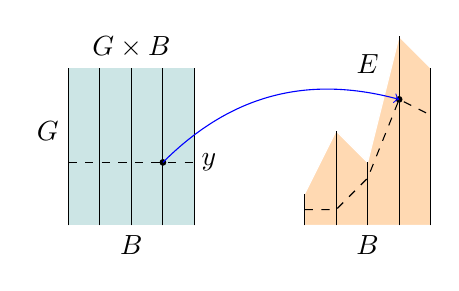
\begin{tikzpicture}
\def\dy{0.2};
\def\yb{0};
\def\yt{10 * \dy}; 

\def\dx{0.4};
\def\xl{-2};
\def\xr{1};

\filldraw[fill=blue!50!green!20, draw=white] (\xl, \yb) rectangle (\xl + 4 * \dx, \yt);
\draw (\xl, \yb) -- (\xl, \yt);
\draw (\xl + \dx, \yb) -- (\xl + \dx, \yt);
\draw (\xl + 2 * \dx, \yb) -- (\xl + 2 * \dx, \yt);
\draw (\xl + 3 * \dx, \yb) -- (\xl + 3 * \dx, \yt);
\draw (\xl + 4 * \dx, \yb) -- (\xl + 4 * \dx, \yt);
\node[below] at (\xl + 2 * \dx, \yb) {$B$};
\node[left] at (\xl + 5 * \dx,  4 * \dy) {$y$};
\node[left] at (\xl,  6 * \dy) {$G$};
\node[above] at (\xl + 2*\dx, 10 * \dy) {$G \times B$};

\def\a{2* \dy}
\def\b{6* \dy}
\def\c{4* \dy}
\def\d{12* \dy}
\def\e{10* \dy}


\draw[fill=orange!30, draw=white] (\xr, \yb) -- (\xr, \a) -- (\xr + 1 * \dx, \b) -- (\xr + 2 * \dx, \c) -- (\xr + 3 * \dx, \d) -- (\xr + 4 * \dx, \e) -- (\xr + 4 * \dx, \yb) -- cycle;


\draw (\xr, \yb) -- (\xr, \a);
\draw (\xr + \dx, \yb) -- (\xr + \dx, \b);
\draw (\xr + 2 * \dx, \yb) -- (\xr + 2 * \dx, \c);
\draw (\xr + 3 * \dx, \yb) -- (\xr + 3 * \dx, \d);
\draw (\xr + 4 * \dx, \yb) -- (\xr + 4 * \dx, \e);

\node[below] at (\xr + 2 * \dx, \yb) {$B$};
\node[above] at (\xr + 2 * \dx, 9 * \dy) {$E$};

\draw[dashed] (\xr, \a -\dy ) -- (\xr + 1 * \dx, \b - 5 * \dy) -- (\xr + 2 * \dx, \c - \dy) -- (\xr + 3 * \dx, \d - 4*\dy) -- (\xr + 4 * \dx, \e - 3*\dy);


\filldraw[black] (\xl + 3 * \dx, \yb + 4* \dy) circle (1 pt);
\filldraw[black] (\xr + 3 * \dx, \yb + 8* \dy) circle (1 pt);

\draw[blue] ((\xl + 3 * \dx, \yb + 4* \dy) edge[->, bend left] (\xr + 3 * \dx, \yb + 8* \dy);

\draw[dashed] (\xl, \yb + 4* \dy) -- (\xl + 4* \dx, \yb + 4* \dy);

\end{tikzpicture}
\]

The adjunction tells us that this family of mappings uniquely determines a function from $G$ to $S(E)$. Every $y \in G$ is thus mapped to a different element $s$ of $S(E)$. Therefore elements of $S(E)$ are in one-to-one correspondence with sections of $E$ .

These are all set-theoretical intuitions. We can generalize them by first noticing that the right hand side of the adjunction can be easily expressed as a hom-set in the slice category $\mathcal{C}/1$ over the terminal object. 

Indeed, there is one-to-one correspondence between objects $X$ in $\mathcal{C}$ and objects $\langle X, ! \rangle$ in  $\mathcal{C}/1$ (here $!$ is the unique arrow to the terminal object). Arrows in $\mathcal{C}/1$ are arrows of $\mathcal{C}$ with no additional constraints. We therefore have:
\[(\mathcal{C}/B) \left( \left \langle {G\times B \atop \pi_2} \right \rangle , \left \langle {E \atop p } \right \rangle \right) \cong (\mathcal{C}/1)  \left( \left \langle {G \atop !} \right \rangle , \left \langle {S(E) \atop ! } \right \rangle \right)  \]

\subsection{Adding the atlas}

The next step is to ``blur the focus'' by replacing the terminal object with a more general base $A$, serving as the atlas.

The right-hand side of the adjunction becomes a hom-set in the slice category $\mathcal{C}/A$. $G$ itself gets coarsely fibrated by some $q \colon G \to A$. 

Remember that $G \times B$ can be understood as a pullback along the mapping $! \colon B \to 1$, or a change of base from $1$ to $B$. If we want to replace $1$ with $A$, we should replace the product $G \times B$ with a more general pullback of $q$. Such a change of base is parameterized by a new morphism $f \colon B \to A$.

\[
 \begin{tikzcd}
 G \times B
 \arrow[dr, phantom,  , very near start, "\lrcorner"]
\arrow[d, "\pi_2"]
 \arrow[r, "\pi_1"]
 & G
 \arrow[d, "!"]
 \\
 B
 \arrow[r, "!"]
 &
 1
 \end{tikzcd}
 \hspace{20pt}
\begin{tikzpicture}
\draw[->] (0, 0) -- (1, 0);
\end{tikzpicture}
 \hspace{20pt}
 \begin{tikzcd}
 f^* G
\arrow[dr, phantom,  , very near start, "\lrcorner"]
 \arrow[d, "f^*q"']
 \arrow[r, "g"]
 & G
 \arrow[d, "q"]
 \\
 B
 \arrow[r, "f"]
 &A
\end{tikzcd}
\]

The result is that, instead of a bunch of $G$ fibers over $B$, we get a pullback $f^* G$ that is populated by groups of fibers from the fibration $q \colon G \to A$. This way $A$ serves as an atlas that enumerates all the patches populated by uniform fibers. 

Imagine, for instance, that $A$ is a two-element set. The fibration $q$ will split $G$ into two fibers. They will serve as our generic fibers. These fibers are now replanted over the two patches in $B$ to form $f^* G$. The replanting is guided by $f^{-1}$. 

\[
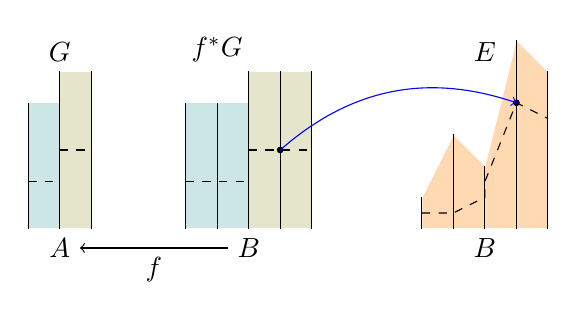
\begin{tikzpicture}
\def\xmin{-4};

\def\dy{0.2};
\def\yb{0};
\def\yt{10 * \dy}; 

\def\dx{0.4};
\def\xl{-2};
\def\xr{1};

\filldraw[fill=blue!50!green!20, draw=white] (\xmin, \yb) rectangle (\xmin + \dx, \yt - 2*\dy);
\filldraw[fill=red!50!green!20, draw=white] (\xmin + \dx, \yb) rectangle (\xmin + 2 * \dx, \yt);
\draw (\xmin, \yb) -- (\xmin, \yt - 2*\dy);
\draw (\xmin + \dx, \yb) -- (\xmin+ \dx, \yt);
\draw (\xmin + 2 * \dx, \yb) -- (\xmin + 2 * \dx, \yt);
\node[below] (BB) at (\xmin + \dx, \yb) {$A$};
\node[above] at (\xmin + \dx, 10 * \dy) {$G$};



\filldraw[fill=blue!50!green!20, draw=white] (\xl, \yb) rectangle (\xl + 4 * \dx, \yt - 2*\dy);
\filldraw[fill=red!50!green!20, draw=white] (\xl + 2 * \dx, \yb) rectangle (\xl + 4 * \dx, \yt);
\draw (\xl + 0 * \dx, \yb) -- (\xl + 0 * \dx, \yt - 2 * \dy);
\draw (\xl + 1 * \dx, \yb) -- (\xl + 1 * \dx, \yt - 2 * \dy);
\draw (\xl + 2 * \dx, \yb) -- (\xl + 2 * \dx, \yt);
\draw (\xl + 3 * \dx, \yb) -- (\xl + 3 * \dx, \yt);
\draw (\xl + 4 * \dx, \yb) -- (\xl + 4 * \dx, \yt);
\node[below] (B) at (\xl + 2 * \dx, \yb) {$B$};
\node[above] at (\xl + \dx, 10 * \dy) {$f^* G$};

\draw[->]  (B) -- (BB) node [midway, below] {$f$};

\def\a{2* \dy}
\def\b{6* \dy}
\def\c{4* \dy}
\def\d{12* \dy}
\def\e{10* \dy}


\draw[fill=orange!30, draw=white] (\xr, \yb) -- (\xr, \a) -- (\xr + 1 * \dx, \b) -- (\xr + 2 * \dx, \c) -- (\xr + 3 * \dx, \d) -- (\xr + 4 * \dx, \e) -- (\xr + 4 * \dx, \yb) -- cycle;


\draw (\xr, \yb) -- (\xr, \a);
\draw (\xr + \dx, \yb) -- (\xr + \dx, \b);
\draw (\xr + 2 * \dx, \yb) -- (\xr + 2 * \dx, \c);
\draw (\xr + 3 * \dx, \yb) -- (\xr + 3 * \dx, \d);
\draw (\xr + 4 * \dx, \yb) -- (\xr + 4 * \dx, \e);

\node[below] at (\xr + 2 * \dx, \yb) {$B$};
\node[above] at (\xr + 2 * \dx, 10 * \dy) {$E$};

% dashed zigzag in E
\draw[dashed] (\xr, \a -\dy ) -- (\xr + 1 * \dx, \b - 5 * \dy) -- (\xr + 2 * \dx, \c - 2* \dy)  -- (\xr + 2 * \dx, \c - \dy) -- (\xr + 3 * \dx, \d - 4*\dy) -- (\xr + 4 * \dx, \e - 3*\dy);

\filldraw[black] (\xl + 3 * \dx, \yb + 5* \dy) circle (1 pt);
\filldraw[black] (\xr + 3 * \dx, \yb + 8* \dy) circle (1 pt);

% arrow from f*G to E
\draw[blue] ((\xl + 3 * \dx, \yb + 5* \dy) edge[->, bend left] (\xr + 3 * \dx, \yb + 8* \dy);

% dashed slices through f*G
\draw[dashed] (\xl, \yb + 3* \dy) -- (\xl + 2 * \dx, \yb + 3* \dy);
\draw[dashed] (\xl + 2 * \dx, \yb + 5* \dy) -- (\xl + 4* \dx, \yb + 5* \dy);

% slices through G
\draw[dashed] (\xmin, \yb + 3* \dy) -- (\xmin + \dx, \yb + 3* \dy);
\draw[dashed] (\xmin + \dx, \yb + 5* \dy) -- (\xmin + 2 * \dx, \yb + 5* \dy);

\end{tikzpicture}
\]

The adjunction that defines the dependent function type is therefore:
\[ (\mathcal{C}/B) \left( f^* \left \langle {G \atop q} \right \rangle, \left \langle {E \atop p} \right \rangle \right) \cong  (\mathcal{C}/A)\left( \left \langle {G \atop q} \right \rangle, \Pi_f \left \langle {E \atop p } \right \rangle \right) \]
This is a generalization of an adjunction that we used to define the object of sections $S(E)$. This one defines a new object $\Pi_f E$ that is a rearrangement of the object of sections. 

The adjunction is a mapping between morphisms in their respective slice categories:

\[
 \begin{tikzcd}
 f^* G
 \arrow[rr, "\phi"]
 \arrow[rd, "f^* q"']
 &&E
 \arrow[dl, "p"]
 \\
 &B
 \end{tikzcd}
 \hspace{20pt}
\begin{tikzcd}
 G
 \arrow[rr, "\phi^T"]
 \arrow[rd, "q"']
 && \Pi_f E
 \arrow[ld, "\Pi_f \, p"]
 \\
 & A
  \end{tikzcd}
\]

To gain some intuition into this adjunction, let's consider how it works on sets. 

\begin{itemize}
\item The right hand side operates in a coarsely grained fibration over the atlas $A$. It is a family of functions, one function per patch. For every patch we get a function from the ``thick fiber'' of $G$ (drawn in blue below) to the ``thick fiber'' of $\Pi_f E$ (not shown).

\item The left hand side operates in a more finely grained fibration over $B$. These fibers are grouped into small bundles over patches. Once we pick a patch (drawn in red below), we get a family of functions from that patch to the corresponding patch in $E$ (drawn in green)---a section of a small bundle in $E$. So, patch-by-patch, we get small sections of $E$. 
\end{itemize}
The adjunction tells us that the elements of the ``thick fiber'' of $\Pi_f E$ correspond to small sections of $E$ over the same patch.

\[
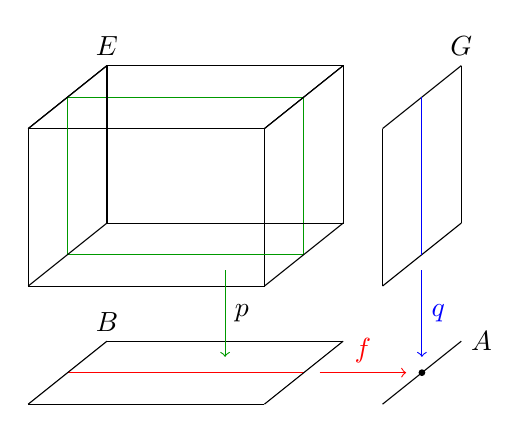
\begin{tikzpicture}
\def\xl{-3};
\def\xr{0};
\def\yb{0};
\def\yt{2};

\def\dy{0.4};
\def\dx{0.5};

\def\a{(\xl, \yb)};
\def\b{(\xr, \yb)};
\def\c{(\xl, \yt)};
\def\d {(\xr, \yt)};

% _a second plane
\def\aa{(\xl + \dx, \yb + \dy)};
\def\ba{(\xr + \dx, \yb + \dy)};
\def\ca{(\xl + \dx, \yt + \dy)};
\def\da{(\xr + \dx, \yt + \dy)};

% _b third plane
\def\ab{(\xl + 2*\dx, \yb + 2*\dy)};
\def\bb{(\xr + 2*\dx, \yb + 2*\dy)};
\def\cb{(\xl + 2*\dx, \yt + 2*\dy)};
\def\db{(\xr + 2*\dx, \yt + 2*\dy)};

% shifted walls
\def\yshift{-1.5};
\def\xshift{1.5};


% E
\draw \a rectangle \d;
\draw[draw=black!40!green] \aa rectangle \da;
\draw \ab rectangle \db;

\draw \a -- \ab;
\draw \b -- \bb;
\draw \d -- \db;
\draw \c -- \cb;

\node[above] at \cb {$E$};

% B
% rebase yb (bottom)
\def\yb{\yshift}
% rebase xr (right wall)
\def\xr{0};

\draw \a -- \b;
\draw \ab -- \bb;
\draw[red] \aa -- \ba;
% diagonal
\draw \a -- \ab;
\draw \b -- \bb;
\draw \d -- \db;
\draw \c -- \cb;
\node[above] at \ab {$B$};

% G
% rebase yb (bottom)
\def\yb{0};
% rebase xr (right wall)
\def\xr{\xshift};
\draw \b -- \bb;
\draw \d -- \db;
\draw \b -- \d;
\draw \bb -- \db;
\draw[blue] \ba -- \da;
\node[above] at \db {$G$};

% A
% rebase yb (bottom)
\def\yb{\yshift}
% rebase xr (right wall)
\def\xr{\xshift};

\draw \b -- \bb;
\node[right] at \bb {$A$};
\filldraw[black] \ba circle (1 pt);

%projections
\draw[blue, shorten <=0.2cm, shorten >=0.2cm, ->] (\xshift + \dx, 0 + \dy) -- node[right]{$q$} (\xshift +\dx, \yshift + \dy);

\draw[red, shorten <=0.2cm, shorten >=0.2cm, ->] (0 + \dx, \yshift + \dy) -- node[above]{$f$} (\xshift +\dx, \yshift + \dy);

\draw[draw=black!40!green, shorten <=0.2cm, shorten >=0.2cm, ->] (0 - \dx, 0 + \dy) -- node[right]{$p$} (0 - \dx, \yshift + \dy);

\end{tikzpicture}
\]

In category theory, the dependent product, which is the right adjoint to the base change functor $f^*$, is denoted by $f_*$. For a given $f \colon b \to a$, it's a functor:
\[ f_* \colon \cat C/b \to \cat C/a \]

The following exercises shed some light on the role played by $f$. It can be seen as localizing the sections of $E$ by restricting them to ``neighborhoods'' defined by $f^{-1}$.

\begin{exercise}
Consider what happens when $A$ is a two-element set $\{0, 1\}$ and $f$ maps the whole of $B$ to one element, say $1$. How would you define the function on the right-hand side of the adjunction? What should it do to the fiber over $0$?
\end{exercise}

\begin{exercise}
Let's pick $G$ to be a singleton set $1$, and let $x \colon 1 \to A$ be a fibration that selects an element in $A$. Using the adjunction, show that:
\begin{itemize}
\item $f^* 1$ has two types of fibers: singletons over the elements of $f^{-1} (x)$ and empty sets otherwise. 
\item A mapping $\phi \colon f^* 1 \to E$ is equivalent to a selection of elements, one from each fiber of $E$ over the elements of $f^{-1}(x)$. In other words, it's a partial section of $E$ over the subset $f^{-1}(x)$ of $B$.
\item A fiber of $\Pi_f E$ over a given $x$ is such a partial section. 
\item What happens when $A$ is also a singleton set?
\end{itemize}
\end{exercise}



\subsection{Universal quantification}

The logical interpretation of the dependent product $\Pi_{x : B} \, T(x)$ is a universally quantified proposition. An element of $\Pi_{x : B} \, T(x)$ is a section---the proof that it's possible to select an element from each member of the family $T(x)$. It means that none of them is empty. In other words, it's a proof of the proposition:
\[ \forall_{x : B}\, T(x) \]

\section{Equality}

Our first experience in mathematics involves equality. We learn that 
\[1+1=2\] 
and we don't think much of it afterwards. 

But what does it mean that $1+1$ is equal to $2$? Two is a number, but one plus one is an expression, so they are not the same thing. There is some mental processing that we have to perform before we pronounce these two things equal. 

Contrast this with the statement $0 = 0$, in which both sides of equality are \emph{the same thing}. 

It makes sense that, if we are to define equality, we'll have to at least make sure that everything is equal to itself. We call this property \emph{reflexivity}. 

Recall our definition of natural numbers:
\begin{haskell}
data Nat where
  Z :: Nat
  S :: Nat -> Nat
\end{haskell}

This is how we can define equality for natural numbers:
\begin{haskell}
equal :: Nat -> Nat -> Bool
equal Z Z = True
equal (S m) (S n) = equal m n
equal _ _ = False
\end{haskell}
We are recursively stripping $S$'s in each number until one of them reaches $Z$. If the other reaches $Z$ at the same time, we pronounce the numbers we started with to be equal, otherwise they are not. 

\subsection{Equational reasoning}

Notice that, when defining equality in Haskell, we were already using the equal sign. For instance, the equal sign in:
\begin{haskell}
equal Z Z = True
\end{haskell}
tells us that wherever we see the expression \hask{equal Z Z} we can replace it with \hask{True} and vice versa. 

This is the principle of substituting equals for equals, which is the basis for \emph{equational reasoning} in Haskell. We can't encode proofs of equality directly in Haskell, but we can use equational reasoning to reason about Haskell programs. This is one of the main advantages of pure functional programming. You can't perform such substitutions in imperative languages, because of side effects.

If we want to prove that $1+1$ is $2$, we have to first define addition. The definition can either be recursive in the first or in the second argument. This one recurses in the second argument:
\begin{haskell}
add :: Nat -> Nat -> Nat
add n Z = n
add n (S m) = S (add n m)
\end{haskell}
We encode $1 + 1$ as:
\begin{haskell}
add (S Z) (S Z)
\end{haskell}
We can now use the definition of \hask{add} to simplify this expression. We try to match the first clause, and we fail, because \hask{S Z} is not the same as \hask{Z}. But the second clause matches. In it, \hask{n} is an arbitrary number, so we can substitute \hask{S Z} for it, and get:
\begin{haskell}
add (S Z) (S Z) = S (add (S Z) Z)
\end{haskell}
In this expression we can perform another substitution of equals using the first clause of the definition of \hask{add} (again, with \hask{n} replaced by \hask{S Z}):
\begin{haskell}
add (S Z) Z = (S Z)
\end{haskell}
We arrive at:
\begin{haskell}
add (S Z) (S Z) = S (S Z)
\end{haskell}
We can clearly see that the right-hand side is the encoding of $2$. But we haven't shown that our definition of equality is reflexive so, in principle, we don't know if
\begin{haskell}
eq (S (S Z)) (S (S Z))
\end{haskell}
yields \hask{True}. We have to use step-by-step equational reasoning again:
\begin{haskell}
equal (S (S Z) (S (S Z)) =
{- second clause of the definition of equal -}
equal (S Z) (S Z) =
{- second clause of the definition of equal -}
equal Z Z =
{- first clause of the definition of equal -}
True
\end{haskell}

We can use this kind of reasoning to prove statements about concrete numbers, but we run into problems when reasoning about generic numbers---for instance, showing that something is true for all \hask{n}. Using our definition of addition, we can easily show that \hask{add n Z} is the same as \hask{n}. But we can't prove that \hask{add Z n} is the same as \hask{n}. The latter proof requires the use of induction. 

We end up distinguishing between two kinds of equality. One is proven using substitutions, or rewriting rules, and is called \emph{definitional equality}. You can think of it as macro expansion or inline expansion in programming languages. It also involves $\beta$-reductions: performing function application by replacing formal parameters by actual arguments, as in:
\begin{haskell}
(\x -> x + x) 2 =
{- beta reduction -}
2 + 2
\end{haskell}

The second more interesting kind of equality is called \emph{propositional equality} and it may require actual proofs. 

\subsection{Equality vs isomorphism}

We said that category theorists prefer isomorphism over equality---at least when it comes to objects. It is true that, within the confines of a category, there is no way to differentiate between isomorphic objects. In general, though, equality is stronger than isomorphism. This is a problem, because it's very convenient to be able to substitute equals for equals, but it's not always clear that one can substitute isomorphic for isomorphic. 

Mathematicians have been struggling with this problem, mostly trying to modify the definition of isomorphism---but a real breakthrough came when they decided to simultaneously weaken the definition of equality. This led to the development of \emph{homotopy type theory}, or HoTT for short. 

Roughly speaking, in type theory, specifically in Martin-L{\"o}f theory of dependent types, equality is represented as a type, and in order to prove equality one has to construct an element of that type---in the spirit of the Curry-Howard interpretation. 

Furthermore, in HoTT, the proofs themselves can be compared for equality, and so on ad infinitum. You can picture this by considering proofs of equality not as points but as some abstract paths that can be morphed into each other; hence the language of homotopies.

In this setting, instead of isomorphism, which involves strict equalities of arrows:
\[ f \circ g = id \]
\[ g \circ f = id \]
one defines an \emph{equivalence}, in which these equalities are treated as types.

The main idea of HoTT is that one can impose the \emph{univalence axiom} which, roughly speaking, states that equalities are equivalent to equivalences, or symbolically:
\[ (A = B) \cong (A \cong B) \]
Notice that this is an axiom, not a theorem. We can either take it or leave it and the theory is still valid (at least we think so).
\subsection{Equality types}

Suppose that you want to compare two terms for equality. The first requirement is that both terms be of the same type. You can't compare apples with oranges. Don't get confused by some programming languages allowing comparisons of unlike terms: in every such case there is an implicit conversion involved, and the final equality is always between same-type values. 

For every pair of values there is, in principle, a separate type of proofs of equality. There is a type for $0 = 0$, there is a type for $1=1$, and there is a type for $1 = 0$; the latter hopefully uninhabited. 

Equality type, a.k.a., identity type, is therefore a dependent type: it depends on the two values that we are comparing. It's usually written as $\text{Id}_A$, where $A$ is the type of both values, or using an infix notation as $x=_A y$ (equal sign with the subscript $A$). 

For instance, the type of equality of two zeros is written as $\text{Id}_{\mathbb{N}} (0, 0)$ or:
\[ 0 =_{\mathbb{N}} 0 \]
Notice: this is not a statement or a term. It's a \emph{type}, like \hask{Int} or \hask{Bool}. You can define a value of this type if you have an introduction rule for it.

\subsection{Introduction rule}

The introduction rule for the equality type is the dependent function: 
\[ \text{refl}_A \colon \Pi_{x : A}  \text{Id}_A  (x, x)\]
which can be interpreted in the spirit of propositions as types as the proof of the statement:
\[ \forall _{x:A} \;x = x \]
This is the familiar reflexivity: it shows that, for all $x$ of type $A$, $x$ is equal to itself. You can apply this function to some concrete value $x$ of type $A$, and it will produce a new value of type $\text{Id}_A  (x, x)$.

We can now prove that $0=0$. We can execute $\text{refl}_{\mathbb{N}} (0)$ to get a value of the type $0 =_{\mathbb{N}} 0$. This value is the proof that the type is inhabited, and therefore corresponds to a true proposition.

This is the only introduction rule for equality, so you might think that all proofs of equality boil down to ``they are equal because they are the same.'' Surprisingly, this is not the case. 

\subsection{$\beta$-reduction and $\eta$-conversion}

In type theory we have this interplay of introduction and elimination rules that essentially makes them the inverse of each other. 

Consider the definition of a product. We introduce it by providing two values, $x \colon A$ and $y \colon B$ and we get a value $p \colon A \times B$. We can then eliminate it by extracting two values using two projections. But how do we know if these are the same values that we used to construct it? This is something that we have to postulate. We call it the computation rule or the $\beta$-reduction rule.

Conversely, if we are given a value $p \colon A \times B$, we can extract the two components using projections, and then use the introduction rule to recompose it. But how do we know that we'll get the same $p$? This too has to be postulated. This is sometimes called the uniqueness condition, or the $\eta$-conversion rule.

In the categorical model of type theory these two rules follow from the universal construction. 

The equality type also has the elimination rule, which we'll discuss shortly, but we don't impose the uniqueness condition. It means that it's possible that there are some equality proofs that were not obtained using $\text{refl}$. 

This is exactly the weakening of the notion of equality that makes HoTT interesting to mathematicians.

\subsection{Induction principle for natural numbers}

Before formulating the elimination rule for equality, it's instructive to first discuss a simpler elimination rule for natural numbers. We've already seen such rule describing primitive recursion. It allowed us to define recursive functions by specifying a value $\mathit{init}$ and a function $\mathit{step}$.

Using dependent types, we can generalize this rule to define the \emph{dependent elimination rule} that is equivalent to the principle of mathematical induction.

The principle of induction can be described as a device to prove, in one fell swoop, whole families of propositions indexed by natural numbers. For instance, the statement that \hask{add Z n} is equal to \hask{n} is really an infinite number of propositions, one per each value of \hask{n}. 

We could, in principle, write a program that would meticulously verify this statement for a very large number of cases, but we'd never be sure if it holds in general. There are some conjectures about natural numbers that have been tested this way using computers but, obviously, they can never exhaust an infinite set of cases.

Roughly speaking, we can divide all mathematical theorems into two groups: the ones that can be easily formulated and the ones whose formulation is complex. They can be further subdivided into the ones whose proofs are simple, and the ones that are hard or impossible to prove. For instance, the famous Fermat's Last Theorem was extremely easy to formulate, but its proof required some massively complex mathematical machinery. 

Here, we are interested in theorems about natural numbers that are both easy to formulate and easy to prove. We'll assume that we know how to generate a family of propositions or, equivalently, a dependent type $T(n)$, where $n$ is a natural number. 

We'll also assume that we have a value:
\[\mathit{init} \colon T(Z) \]
or, equivalently, the proof of the zeroth proposition; and a dependent function:
\[\mathit{step} \colon \Pi_{n:\mathbb{N}}\,\left(T(n) \to T(S n)\right) \]
This function is interpreted as generating a proof of the $(n + 1)$st proposition from the proof of the $n$th proposition.

The \emph{dependent elimination rule} for natural numbers postulates that, given such $\mathit{init}$ and $\mathit{step}$, there exists a dependent function:
\[f \colon \Pi_{n:\mathbb{N}} \, T(n) \]
This function is interpreted as providing the proof that $T(n)$ is true for all $n$.

Moreover, this function, when applied to zero reproduces $\mathit{init}$:
\[ f (Z) = \mathit{init} \]
and, when applied to the successor of $n$, is consistent with taking a $\mathit{step}$:
\[ f (S n) = (\mathit{step} (n)) (f (n)) \]
(Here, $\mathit{step}(n)$ produces a function, which is then applied to the value $f(n)$.) These are the two \emph{computation rules} for natural numbers. 

Notice that the induction principle is not a theorem about natural numbers. It's part of the \emph{definition} of the type of natural numbers. 

Not all dependent mappings out of natural numbers can be decomposed into $\mathit{init}$ and $\mathit{step}$, just as not all theorems about natural numbers can be proven inductively. There is no $\eta$-conversion rule for natural numbers.

\subsection{Equality elimination rule}

The elimination rule for equality type, also called the \index{J-rule}J-rule, is somewhat analogous to the induction principle for natural numbers. There we used $\mathit{init}$ to ground ourselves at the start of the journey, and $\mathit{step}$ to make progress. The elimination rule for equality requires a more powerful grounding, but it doesn't have a $\mathit{step}$. There really is no good analogy for how it works, other than through a leap of faith.

The idea is that we want to construct a mapping \emph{out} of the equality type. But since equality type is itself a two-parameter family of types, the mapping out should be a dependent function. The target of this function is another family of types:
\[T(x, y, p)\]
 that depends on the pair of values that are being compared $x, y \colon A$, and the proof of equality $p \colon \text{Id}(x, y)$.
 
 The function we are trying to construct is:
 \[ f \colon \Pi_{x, y : A} \Pi_{p : \text{Id}(x, y)} \, T(x, y, p) \]

It's convenient to think of it as generating a proof that for all points $x$ and $y$, and for every proof that the two are equal, the proposition $T(x, y, p)$ is true. Notice that, potentially, we have a different proposition for \emph{every proof} that the two points are equal.

The least that we can demand from $T(x, y, p)$ is that it should be true when $x$ and $y$ are literally the same, and the equality proof is the obvious $\text{refl}$. This requirement can be expressed as a dependent function:
\[t \colon \Pi_{x : A} \,T\left(x, x, \text{refl}(x)\right)\]
Notice that we are not even considering proofs of $x = x$, other than those given by reflexivity. Do such proofs exist? We don't know and we don't care.

So this is our grounding, the starting point of a journey that should lead us to defining our $f$ for all pairs of points and all proofs of equality. The intuition is that we are defining $f$ as a function on a plane $(x, y)$, with a third dimension given by $p$. To do that, we're given something that's defined on the diagonal $(x, x)$, with $p$ restricted to $\text{refl}$.

\[
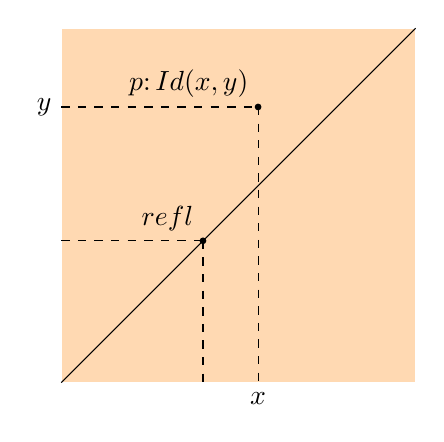
\begin{tikzpicture}

\def\yb{0}; 
\def\ydiag{1.8};
\def\yoff{3.5};
\def\yt{4.5}; 


\def\xl{0};
\def\xdiag{\ydiag};
\def\xoff{2.5};
\def\xr{\yt};

\filldraw[fill=orange!30, draw=white] (\xl, \yb) rectangle (\xr, \yt);

\draw (\xl, \yb) -- (\xr, \yt); % diagonal

\draw[dashed] (\xdiag, \ydiag) -- (\xdiag, \yb);
\draw[dashed] (\xl, \ydiag) -- (\xdiag, \ydiag);

\filldraw[black] (\xdiag, \ydiag) circle (1 pt);
\node[above left] at (\xdiag, \ydiag) {$\text{refl}$};

\draw[dashed] (\xoff, \yoff) -- (\xoff, \yb);
\draw[dashed] (\xl, \yoff) -- (\xoff, \yoff);

\filldraw[black] (\xoff, \yoff) circle (1 pt);
\node[above left] at (\xoff, \yoff) {$p\colon \text{Id}(x, y)$};

\node[below] at (\xoff, \yb) {$x$};
\node[left] at (\xl, \yoff) {$y$};

\end{tikzpicture}
\]

You would think that we need something more, some kind of a $\mathit{step}$ that would move us from one point to another. But, unlike with natural numbers, there is no \emph{next} point or \emph{next} equality proof to jump to. All we have at our disposal is the function $t$ and nothing else. 

Therefore we postulate that, given a type family $T(x, y, p)$ and a function:
\[t \colon \Pi_{x : A} \,T\left(x, x, \text{refl}(x)\right)\]
there exists a function:
 \[ f \colon \Pi_{x, y : A} \Pi_{p : \text{Id}(x, y)} \, T(x, y, p) \]
such that (computation rule):
\[f (x, x, \text{refl}(x)) = t(x)\]
Notice that the equality in the computation rule is \emph{definitional equality}, not a type.

Equality elimination tells us that it's always possible to extend the function $t$, which is defined on the diagonal, to the whole 3-d space. 

This is a very strong postulate. One way to understand it is to argue that, within the framework of type theory---which is formulated using the language of introduction and elimination rules, and the rules for manipulating those---it's \emph{impossible} to define a type family $T(x, y, p)$ that would \emph{not} satisfy the equality elimination rule. 

The closest analogy that we've seen so far is the result of parametricity, which states that, in Haskell, all polymorphic functions between endofunctors are automatically natural transformations. Another example, this time from calculus, is that any analytic function defined on the real axis has a unique extension to the whole complex plane. 

The use of dependent types blurs the boundary between programming and mathematics. There is a whole spectrum of languages,  starting with Haskell barely dipping its toes in dependent types while still firmly established in commercial usage, all the way to theorem provers, which are helping mathematicians formalize mathematical proofs.

\end{document}